\documentclass[12pt,letterpaper,final]{article}

\usepackage{Sweave}
\usepackage{graphicx}
\usepackage{natbib}
\usepackage{hyperref}
\usepackage{caption}
\usepackage{rotating}
\usepackage{verbatim}
\usepackage{textcomp}
%\usepackage[hyphens]{url}
\usepackage{latexsym}
\usepackage{wasysym}

\setlength{\oddsidemargin}{0in}
\setlength{\textwidth}{6.15in}
%\setlength{\topmargin}{0.5in}
\setlength{\textheight}{22cm}
\setlength{\headheight}{0in}
\setlength{\headsep}{0in}
\setlength{\parskip}{5pt plus 2pt minus 3pt}

\def\thefootnote{\fnsymbol{footnote}}
\setcounter{footnote}{1}

\renewcommand{\baselinestretch}{1.2}\renewcommand{\labelenumi}{(\roman{enumi})}

\renewcommand{\topfraction}{1.0}
\renewcommand{\bottomfraction}{1.0}
\renewcommand{\textfraction}{0.0}
\renewcommand{\floatpagefraction}{1.0}

\newtheorem{definition}{Definition}
\newtheorem{theorem}{Theorem}
\newtheorem{lemma}[theorem]{Lemma}
\newtheorem{claim}[theorem]{Claim}
\newtheorem{fact}[theorem]{Fact}

% to get nice proofs ...
\newcommand{\qedsymb}{\mbox{ }~\hfill~{\rule{2mm}{2mm}}}
\newenvironment{proof}{\begin{trivlist}
\item[\hspace{\labelsep}{\bf\noindent Proof: }]
}{\qedsymb\end{trivlist}}


\newfont{\msymb}{cmsy10 scaled 1000}

\def\nullset{\mbox{\O}}
\def\R{{I\!\!R}}
\def\C{{I\!\!\!\!C}}
\def\N{{I\!\!N}}

\def\P{\mbox{\msymb P}}


%\parskip 0.1in
\pagenumbering{arabic}    %  Start using 1,2,... as page numbers.
\pagestyle{plain}         %  Page numbers in middle bottom of page.
%\setcounter{page}{80}  % XXXXXXXXXXXXXXXXX
%\setcounter{theorem}{5} % XXXXXXXXXXXXXXXXX
%\setcounter{definition}{10} % XXXXXXXXXXXXXXXXX

\parindent 0in


\begin{document}

\Sconcordance{concordance:hw02_bartschi.tex:hw02_bartschi.Rnw:%
1 116 1 1 2 1 0 8 1 3 0 1 2 8 1 1 2 5 0 1 2 11 1 1 2 1 0 1 1 1 5 3 0 1 %
5 3 0 1 5 3 0 1 5 3 0 1 2 4 0 1 2 12 1 1 8 11 0 1 2 9 1 1 2 1 0 1 1 1 2 %
1 0 1 2 1 0 1 2 1 0 1 2 5 0 1 2 17 1 1 13 12 0 1 12 11 0 1 12 11 0 1 12 %
11 0 1 12 11 0 1 12 11 0 1 2 4 0 1 2 17 1 1 6 5 0 1 7 6 0 1 6 5 0 1 1 4 %
0 1 2 13 1 1 5 8 0 1 2 8 1 1 5 8 0 1 2 44 1 1 2 1 0 1 1 4 0 2 2 5 0 2 2 %
5 0 2 2 5 0 2 2 5 0 2 2 5 0 1 2 13 1 1 2 5 0 1 2 26 1 1 2 1 0 1 3 6 0 1 %
2 52 1}


\begin{titlepage}
\vspace*{4.5cm}
\begin{center}
{\LARGE \bf Stat 5810, Section 003} \\[0.5cm]
{\LARGE \bf Statistical Visualization II} \\[0.5cm]
{\LARGE \bf Spring 2019} \\[0.5cm]
{\LARGE \bf Homework 2} \\[0.5cm]
~ \\[2cm]
{\bf ShaunMicheal Bartschi} \\[0.3cm]
{A01975136} \\[0.3cm]
{April 11, 2019} \\[0.3cm]
\end{center}

\thispagestyle{empty}
\vfill
\end{titlepage}


\begin{table}\centering
\begin{tabular*}{6.15in}{@{\extracolsep{\fill}}|llr|} \hline
Stat 5810/6910 Statistical Visualization II  & \hspace*{0.5 in} & Spring 2019 \\
 & & \\
\multicolumn{3}{|c|}{
Homework Assignment 2 (3/29/2019)} \\
 & & \\
\multicolumn{3}{|c|}{
100 Points --- Due Thursday 4/11/2019 (via Canvas by 11:59pm)} \\
\hline
\end{tabular*}
\end{table}


\begin{enumerate}

\item {\bf International Encyclopedia of Statistical Sciences} (25 Points): \\
The {\it International Encyclopedia of
Statistical Sciences} (\url{http://www.springer.com/us/book/9783642048975}),
published in 2011, is a unique world--wide project. The editors were
able to unite 619 authors from 104 different countries --- and
received themselves a nomination for the Nobel Peace Prize in 2011
(see \url{http://magazine.amstat.org/blog/2011/05/01/peace-through-statistics/}
for details).

\begin{enumerate} 
\item (18 Points)
Your task is simple: Reproduce the choropleth map shown in Figure~3 of 
the {\it Amstat News} article. Use the same colors and intervals as
in the original publication

The data are stored in the Excel file \\
\hspace*{2cm}\verb|hw02_Encyclopedia_Frequency_Distribution.xls|. \\
Read the data in directly,
using one of the R packages for Excel, such as \verb|readxl|.
You are not allowed to change the type of this file (e.g., to csv instead of xls).

For the choropleth map, use an R package of your choice. 
I worked with the maps from the {\it maptools} R package originally.
When I created the map for the {\it Amstat News} article in 2011, 
I found this posting very helpful: \\
{\scriptsize
\url{http://r.789695.n4.nabble.com/political-maps-world-maps-in-R-wrld-simpl-td887910.html}. } \\
There may be other, more recent web postings that provide additional help.

Several country names in the Excel file may not match the names that are used
in the R package (think of Great Britain, United Kingdom, U.K., or UK).
You need to figure out yourself which names are not matching and then replace
them in your internal data structure in R (and not in the external Excel file!).
Using R code to determine which names are not matching may be a good idea.

With respect to colors, I have used a 5--class {\it YlGnBu} palette from {\it RColorBrewer}.
I found it easier to write the resulting map into a pdf file and
specify the dimensions for that pdf file, rather than trying to control
the dimensions of the map through R/Markup/Sweave/knitr.
Do not use Photoshop to edit out the small islands and Antarctica.
This was done by someone at ASA after they received my
map with all islands included. \frownie{}
Show your R code for all data manipulations and include your final resulting map.
Again, modifying the external Excel file is not permitted! \\


\underline{Answer}: \\
{\scriptsize
\begin{Schunk}
\begin{Sinput}
> setwd("C:/Users/Shaun/Desktop/StatVis/StatVis2/HW2")
> library(readxl)
> library(maps)
> library(maptools)
> library(RColorBrewer)
> data("wrld_simpl")
> input.data <- read_excel("hw02_Encyclopedia_Frequency_Distribution.xls")
> #Help from https://stackoverflow.com/questions/11254524/
> #Remove the final row which contained the sum of the submissions
> input.data <- input.data[complete.cases(input.data),]
> contributing.countries <- input.data$Country
> contributions <- input.data$`Number of Contributors`
> country.all <- wrld_simpl$NAME # countries' names as coded in wrld_simpl 
> n.all       <- length(country.all) 
> col.map     <- numeric(n.all) 
> patramp <- colorRamp(c(rgb(0,0,.7),"red"))# my personal ramp color palette 
> #This was my method for finding countries which were not mapping correctly.
> bad.pos <- vector(mode="numeric", length=0)
> bad.names <- vector(mode="character", length=0)
> for (i in 1:length(contributing.countries)){ 
+   if(length(levels(country.all)[levels(country.all)==contributing.countries[i]]) == 0){
+     bad.pos <- c(bad.pos,i)
+     bad.names <- c(bad.names,contributing.countries[i])
+   }
+ } 
> #These were the positions of the countries that don't map correctly.
> #bad.pos = c(14,39,44,51,53,59,63,64,93,100,103)
> #These were the names of the countries (from input) that don't map correctly
> #bad.names = c("Bosnia", "Great Britain", "Iran", "Kazahstan", "Korea", "Macedonia",
> #              "Moldova", "Monte Negro", "Trinidad", "USA", Vietnam)
> 
> #Rename countries to proper form
> contributing.countries[contributing.countries == "Bosnia"] <-
+   "Bosnia and Herzegovina"
> contributing.countries[contributing.countries == "Great Britain"] <- 
+   "United Kingdom"
> contributing.countries[contributing.countries == "Iran"] <- 
+   "Iran (Islamic Republic of)"
> contributing.countries[contributing.countries == "Kazahstan"] <- 
+   "Kazakhstan"
> contributing.countries[contributing.countries == "Korea"] <- 
+   "Korea, Republic of" #I presumed N.Korea didn't contribute much
> contributing.countries[contributing.countries == "Macedonia"] <- 
+   "The former Yugoslav Republic of Macedonia"
> contributing.countries[contributing.countries == "Moldova"] <- 
+   "Republic of Moldova"
> contributing.countries[contributing.countries == "Monte Negro"] <- 
+   "Montenegro"
> contributing.countries[contributing.countries == "Trinidad"] <- 
+   "Trinidad and Tobago"
> contributing.countries[contributing.countries == "USA"] <- 
+   "United States"
> contributing.countries[contributing.countries == "Vietnam"] <- 
+   "Viet Nam"
> #check that there are no longer any unmapped values:
> check.map <- TRUE
> for (i in 1:length(contributing.countries)){ 
+   if(length(levels(country.all)[levels(country.all)==contributing.countries[i]]) == 0){
+     check.map <- FALSE
+   }
+ }
> print(check.map)
\end{Sinput}
\begin{Soutput}
[1] TRUE
\end{Soutput}
\begin{Sinput}
> # grep contributing.countries in country.all
> for (i in 1:length(contributing.countries)){
+   col.map[grep(contributing.countries[i],country.all)] <- contributions[i]
+ }
> breaks <- c(-1,0,1,5,10,215)
> m.class <- cut(col.map,breaks)
> m.col <- brewer.pal(5, "YlGnBu")[m.class]
> plot(wrld_simpl,col = m.col,axes=F, 
+      main = "Countries with Authors Contributing the the IESS",
+      xlim = c(-100,100)) # nice plot
> #,xlim = c(0,75), ylim = c(-125,125)
> legend(x = -160, y = 10, legend = c("0","1","2-5","6-10","11-214"), 
+        fill = brewer.pal(5, "YlGnBu"))
\end{Sinput}
\end{Schunk}
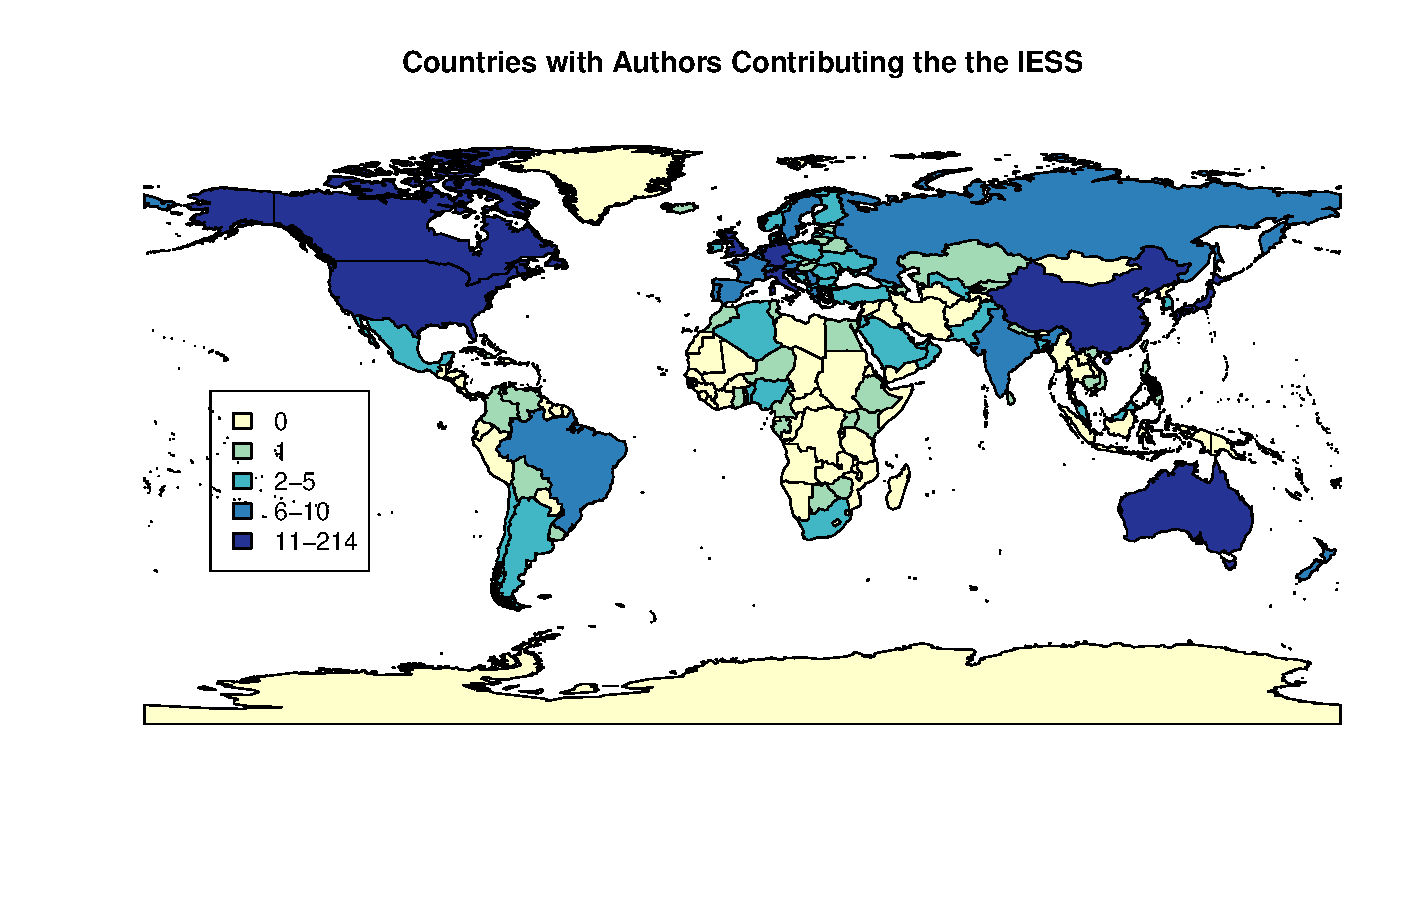
\includegraphics{hw02_bartschi-001}
\\For comparison, here is the original figure from {\it Amstat News}:\\
\begin{center}
  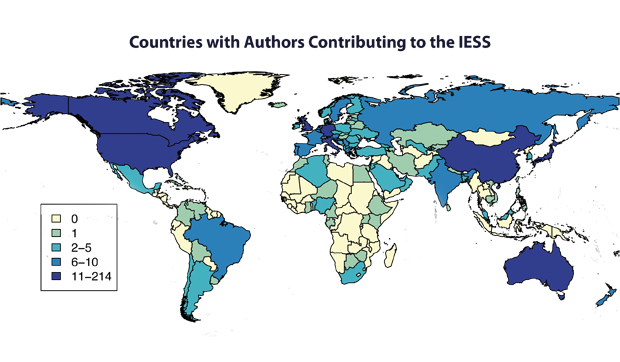
\includegraphics[width=9.5 cm]{original_Contributor_map.png}
\end{center}
}


\item (7 Points)
Write a report that summarizes the main features that are visible in your map.
You may want to comment on
which countries had most contributors overall --- and which
countries had surprisingly many authors, compared to their
neighboring countries. Keep in mind (and remind the reader)
that these are counts and not proportions! \\


\underline{Answer}: \\
{\scriptsize
  This mapping shows which countries had authors who contributed to the IESS project, as well as the frequency (total number) of those contributions.  From the graph, it would appear that the majority of contributions came for North America, Australia, and Europe, with Asia and South America being moderate contributors and Africa being a minor contributor. It is important to note from the legend that the color scale is based only on the number of contributions, as a opposed to the proportion of total contributions.  Furthermore, there is a very wide range for the top color, making it difficult to see that the United States had 214 contributions compared to China's 11 contributions although they share the same color legend.\\
  This map shows that countries like the United States, Canada, Australia, Great Britain, China, Croatia (surprisingly), Germany, Italy, and Japan made the most contributions to the IESS project.  Countries that might be surprising to note as frequent contributors (compared to the relative contributions of their neighbors) are Malaysia, Saudi Arabia, Oman, the U.A.E., Algeria, Brazil, Benin, and Nigeria.
}
\end{enumerate}


\newpage


\item {\bf Alabama First --- Finally!} (25 Points) \\
Alabama was the first state since the 2016 Presidential election
where a special election took place on December 12, 2017, to fill in a United States Senate seat.
Doug Jones, a Democrat, won against Roy S.\ Moore, a Republican, 
making Jones the first Democrat to win a Senate seat in Alabama in over 25 years.
Results at the county level can be obtained from \\
{\scriptsize
\url{https://www.nytimes.com/elections/results/alabama-senate-special-election-roy-moore-doug-jones}.} \\
I am using the R code below to scrape these data from the web:


{\scriptsize
\begin{Schunk}
\begin{Sinput}
> library(httr)
> library(XML)
> page <- GET("https://www.nytimes.com/elections/results/alabama-senate-special-election-roy-moore-doug-jones")
> summary(page)
> # extract the nodes related to the tables
> pagehtml <- htmlParse(page)
> summary(pagehtml)
> nodes <- getNodeSet(pagehtml, "//table")
> nodes
> class(nodes)
> summary(nodes)
> head(nodes[[2]])
> # extract the election table from the page
> etable <- readHTMLTable(nodes[[2]])
> head(etable)
> colnames(etable) <- gsub(" |\n|[-]|[.]", "", colnames(etable))
> etable$JonesNum <- as.integer(gsub(",", "", etable$Jones))
> etable$MooreNum <- as.integer(gsub(",", "", etable$Moore))
> etable$WriteInsNum <- as.integer(gsub(",", "", etable$WriteIns))
> head(etable)
\end{Sinput}
\end{Schunk}
}


\newpage


\begin{enumerate}
\item (2 Points) 
Load all additional R packages you need for this question.
Calculate the percentages for Jones and Moore in each of the 67 counties,
based on all votes (including write--ins) cast in these counties.
Determine the winning percentages for Jones and Moore in each county
and set as NA for the candidate who lost that county. 
Show the first 6 rows of the resulting data frame.
Show your R code. \\


\underline{Answer:}
{\scriptsize
\begin{Schunk}
\begin{Sinput}
> etable$total.votes <- etable$JonesNum + etable$MooreNum + etable$WriteInsNum
> etable$Jones.Pct <- etable$JonesNum / etable$total.votes
> etable$Moore.Pct <- etable$MooreNum / etable$total.votes
> for(i in 1:length(etable$County)){
+   if(etable$Jones.Pct[i] > etable$Moore.Pct[i]){
+     etable$Moore.Pct[i] <- NA
+   } else {
+     etable$Jones.Pct[i] <- NA
+   }
+ }
> head(etable)
\end{Sinput}
\begin{Soutput}
      County   Jones  Moore WriteIns  Rpt JonesNum MooreNum WriteInsNum
1  Jefferson 149,522 66,309    3,710 100%   149522    66309        3710
2    Madison  65,664 46,313    3,446 100%    65664    46313        3446
3     Mobile  62,253 46,725    1,539 100%    62253    46725        1539
4 Montgomery  48,186 17,705      743 100%    48186    17705         743
5     Shelby  27,251 36,424    1,718 100%    27251    36424        1718
6    Baldwin  22,131 38,445    1,699 100%    22131    38445        1699
  total.votes Jones.Pct Moore.Pct
1      219541 0.6810664        NA
2      115423 0.5688987        NA
3      110517 0.5632889        NA
4       66634 0.7231443        NA
5       65393        NA 0.5570015
6       62275        NA 0.6173424
\end{Soutput}
\end{Schunk}
}


\item (3 Points) 
Create side--by--side boxplots for the winning percentages for the 2 candidates
in the 67 counties.
What do you observe? 
There is one interesting feature for one of the counties won by Moore.
Which? Keep in mind that we have write--ins!
Look very carefully or use additional summary statistics.
Answer this part in 3 or 4 sentences and show your R code.\\

\underline{Answer:}
{\scriptsize
\begin{Schunk}
\begin{Sinput}
> boxplot(etable$Jones.Pct,etable$Moore.Pct, horizontal = T,
+         main = "Winning Percentages by Candidate",
+         names = c("Jones", "Moore"), col = c("Blue","Red"))
> summary(etable$Jones.Pct)
\end{Sinput}
\begin{Soutput}
   Min. 1st Qu.  Median    Mean 3rd Qu.    Max.    NA's 
 0.5012  0.5566  0.6107  0.6541  0.7671  0.8814      42 
\end{Soutput}
\begin{Sinput}
> summary(etable$Moore.Pct)
\end{Sinput}
\begin{Soutput}
   Min. 1st Qu.  Median    Mean 3rd Qu.    Max.    NA's 
 0.4994  0.5998  0.6478  0.6638  0.7258  0.8271      25 
\end{Soutput}
\begin{Sinput}
> etable$County[which.min(etable$Moore.Pct)]
\end{Sinput}
\begin{Soutput}
[1] Monroe
67 Levels: Autauga Baldwin Barbour Bibb Blount Bullock Butler ... Winston
\end{Soutput}
\end{Schunk}
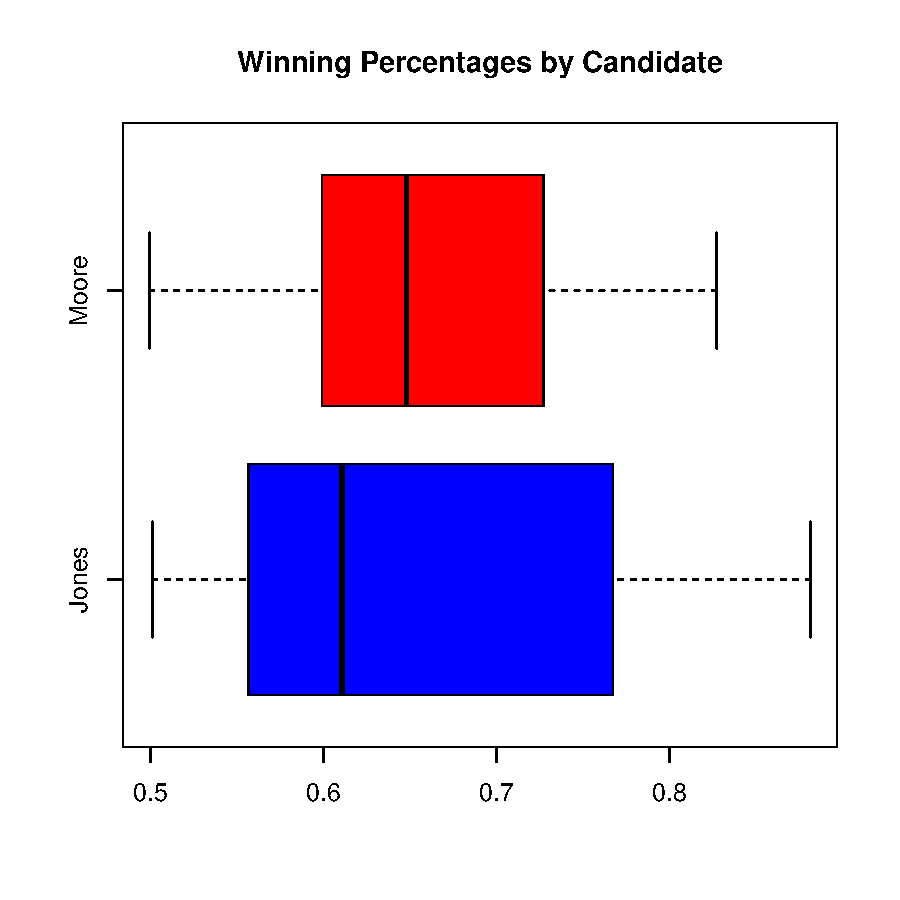
\includegraphics{hw02_bartschi-004}
\\ \underline{\bf Overall Observations:} From the boxplot it appears that Jones had more victories with slimmer margins that Moore did, however Jones also had some victories by larger margins that Moore did.  That is to say that the 2nd Quartile of Moore's victories in the range of 59.9\%-64.7\% was overall larger compared to Jones's 55.6\%-61.0\%, while for the 4th Quartile, Jones's victories were larger, was they were in the range of 76.7\%-88.1\% compared to Moore's 72.5\%-82.7\%.\\
\underline{\bf Interesting Observation:} While it took me a moment to find what particularity was being referred to in the problem statement, I came to realize by looking at the summary statistics that in Monroe County, which Moore had won, he actually had \it{less} than half of the total votes.  After investigating, there was a 33 vote difference between the two candidates, but there were 40 total write-In votes, indicating why Moore won by less than half.
}


\item (15 Points) 
Create a map using the {\it maps} R package, similar to the one shown at \\
{\scriptsize
\url{https://www.nytimes.com/elections/results/alabama-senate-special-election-roy-moore-doug-jones}}. \\
Use darker blue tones for higher winning percentages of Jones and
darker red tones for higher winning percentages of Moore.
Use a 10--class red--blue divergent color scheme
that can be obtained as \verb|brewer.pal(10, "RdBu")| from the {\it RColorBrewer} R package.
Use similar intervals as used by the New York Times, but further improve their intervals
to cover the entire range of the winning percentages.
Do not forget a create a meaningful legend.
Also display the names of the five cities on the map that are shown in the New York Times map.
There exists a {\it map.cities} function in the {\it maps} R package. See the help
page and do some experimentation such that only these five cities are listed by name on the map.
Show your R code. \\


\underline{Answer:}
{\scriptsize
\begin{Schunk}
\begin{Sinput}
> library(maps)
> winning.Pct <- vector(mode="numeric", length=length(etable$County))
> etable.sorted <- etable[order(etable$County),]
> counties <- gsub("alabama,", "", map("county","Alabama", plot = F)$names)
> alabama.breaks <- c(-1,-.73,-.65,-.57,-.49,.49, .57, .65, .73, .81, 1)
> for (i in 1:length(etable$County)){
+   if(is.na(etable.sorted$Jones.Pct[i])){
+     winning.Pct[i] <- -(etable.sorted$Moore.Pct[i])
+   } else{
+     winning.Pct[i] <- etable.sorted$Jones.Pct[i]
+   }
+ }
> m.winning <- cut(winning.Pct, alabama.breaks)
> par(mar=c(5.1, 4.1, 4.1, 8.1), xpd=TRUE)
> map.m.col <- brewer.pal(10, "RdBu")[m.winning]
> map("county", "Alabama", fill = TRUE,
+     col = map.m.col, border = "White")
> title(main = "Alabama 2017 Special Election Results", 
+       xlab = "Color indicates candidate: Blue for Jones, Red for Moore")
> data("us.cities")
> election.towns <- us.cities[
+   us.cities$name %in% 
+     c("Birmingham AL","Huntsville AL","Tuscaloosa AL", "Montgomery AL", "Mobile AL"),]
> election.towns$name <- gsub(" AL", "", election.towns$name)
> map.cities(election.towns, country = "AL")
> map.cities(election.towns, country = "AL", capitals = 2, cex = 0.65)
> legend("right", legend = 
+          c(">81%","73-81%","65-73%","57-65%","<57%",
+            "<57%","57-65%","65-73%","73-81%",">81%"), 
+        fill = brewer.pal(10, "RdBu"), inset = c(-0.56,0), 
+        title = "Winning Vote Share")
\end{Sinput}
\end{Schunk}
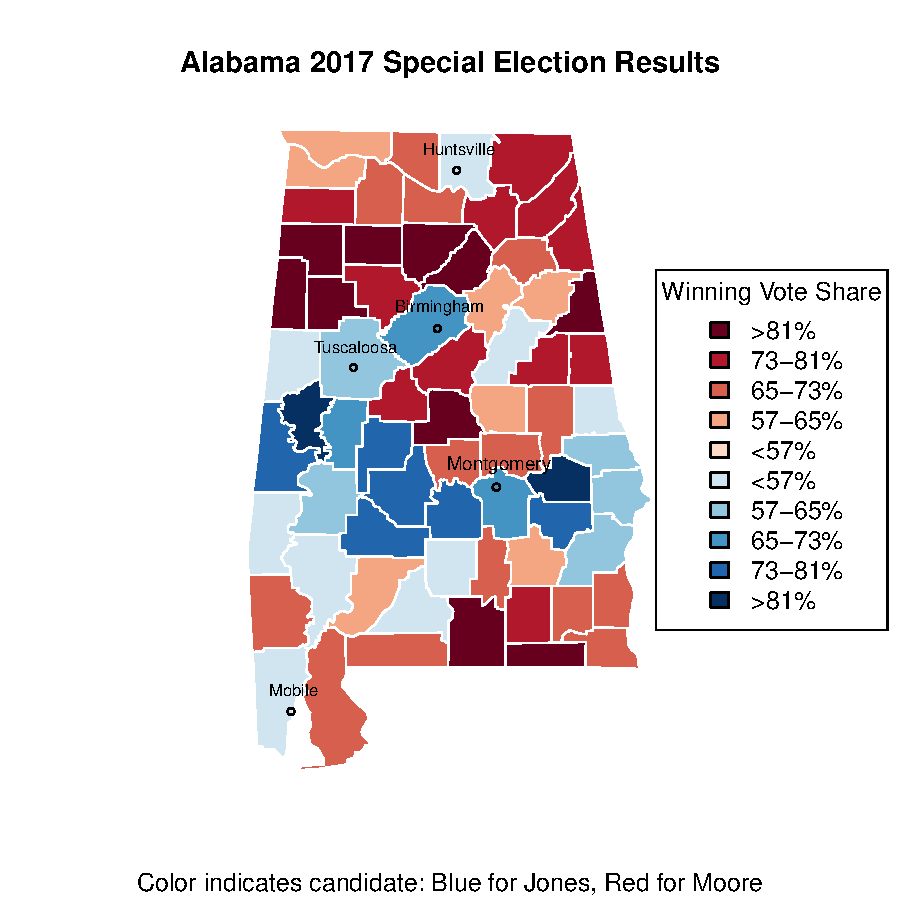
\includegraphics{hw02_bartschi-005}
}


\item (5 Points)
{\bf Carefully compare your map with the map posted at} \\
{\scriptsize
\url{https://www.nytimes.com/elections/results/alabama-senate-special-election-roy-moore-doug-jones}}. \\
If you took {\it Data Technologies} in the fall, you should remember what might go
wrong with geographic data and names from multiple sources. Compare spellings, the order 
how subregions appear in the different sources, etc. Once you are convinced that 
everything is correct in your map,
describe the geographic pattern in the map. Where did Jones win and where did Moore win?
Clearly, if Moore won over Jones in Birmingham or Montgomery, something 
must have gone totally wrong in your map!
It may also be a good idea to look at a real map of Alabama to answer this part. \\


\underline{Answer:} \\
{\scriptsize
After a fair deal of tweaking, I am now confident that my map is an accurate representation of the election results and is comparable with the source graph.\\
It would appear that Moore won more often in the northern and southern regions of Alabama, in fact it seems that Moore won more area in the State than Jones.  The central region seemed to be mostly victories for Jones, and furthermore include all of the five major cities listed by the {\it New York Times}.
}

\end{enumerate}


\newpage


\item {\bf Linked Micromap Plots} (25 Points): \\
In this question, you have to recreate a linked micromap plot from Chapter~4
(``{\it Linked Micromaps}'') in Carr \& Pickle (2010), included in this 
homework as Figure~\ref{fig:OrigFig4.3}. 

\begin{enumerate}
\item (18 Points)
Using the data {\it edPov} data from the {\it micromapST} R package, reproduce
Figure~4.3 from Carr \& Pickle (2010) with the {\it micromap} R package. 
How similar to the original figure can you make your version?
Be specific which features you could not recreate with the {\it micromap} R package.
Show your R code and the final resulting linked micromap plot. \\

\underline{Answer:}
{\scriptsize
\begin{Schunk}
\begin{Sinput}
> library(micromap)
> library(micromapST)
> data(USstates)
> data(edPov)
> stateData <- cbind(as.data.frame(state.x77), State = rownames(state.x77))
> statePolys <- create_map_table(USstates, "ST_NAME")
> BasicPlotb <- mmplot(stat.data = stateData,
+                      map.data = statePolys,
+                      panel.types = c("map", "labels", "dot"),
+                      panel.data = list(NA, "State", "Murder"),
+                      ord.by = "Murder",
+                      grouping = 5,
+                      map.link = c("State", "ID"))
> 
> # 
> # BasicPlot <- mmplot(stat.data = edPov,
> #                     map.data = statePolys, 
> #                     panel.types = c('labels', 'dot', 'dot','map'),
> #                     panel.data = list('state','pov','ed', NA),
> #                     ord.by = "pov",
> #                     grouping = 5,
> #                     # plot.height = 9,
> #                     # plot.width = 5,
> #                     colors = c("red", "blue", "green", "purple", "orange"),
> #                     map.link = c("StateAb", "ID")
> #                     # map.color2 = "lightgray", 
> #                     # 
> #                     # plot.panel.spacing = 0,
> #                     # panel.att = list(
> #                     #    list(1, header = "States",
> #                     #        inactive.border.color = gray(0.7),
> #                     #        inactive.border.size = 1,
> #                     #        panel.width = 0.8),
> #                     #   list(2, header = "Percent living below\npoverty level", 
> #               xaxis.title = 'Percent'),
> #                     #   list(3,header = "Percent adults with\n4+ years of college", 
> #               xaxis.title = 'Percent',,
> #                     #        text.size = 0.7),
> #                     #   list(4, header = "Light gray indicates\nhighlighted above",
> #                     #        header.color = "red",
> #                     #        graph.bgcolor = "lightgray",
> #                     #        point.size = 1,
> #                     #        xaxis.ticks = seq(0, 16, by = 4),
> #                     #        xaxis.labels = seq(0, 16, by = 4)
> #                     #        )
> #                     # )
> # )
> 
\end{Sinput}
\end{Schunk}
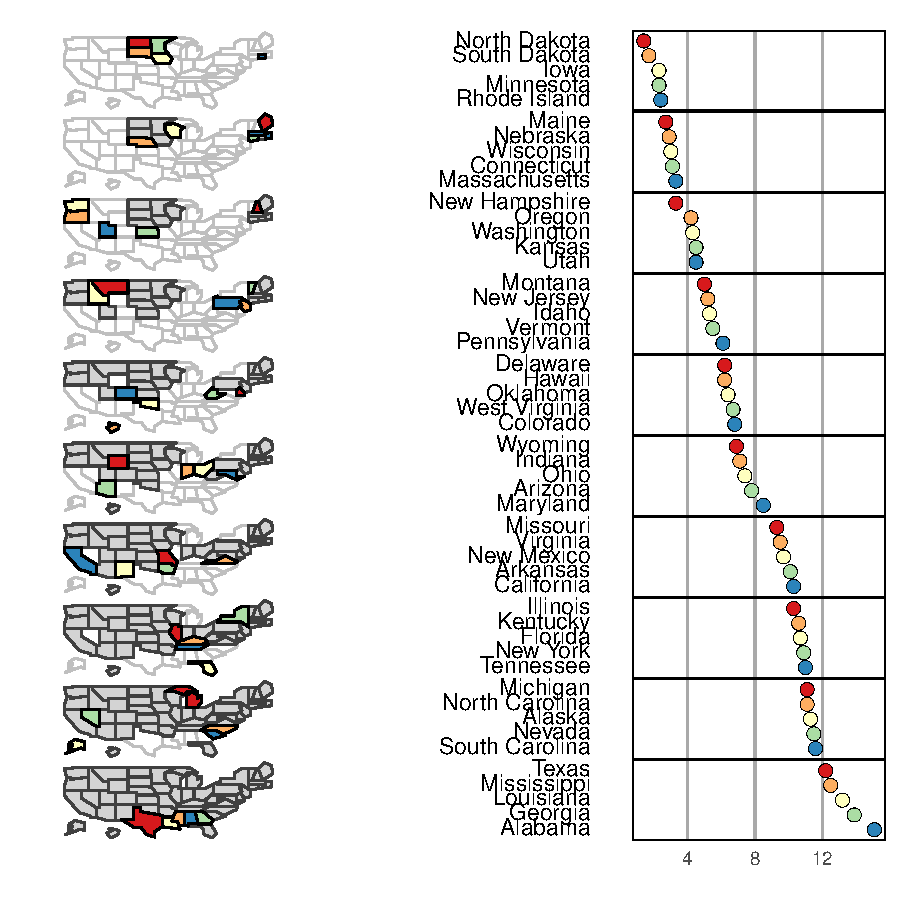
\includegraphics{hw02_bartschi-006}
\\ I was having some trouble getting my micromap to work.  I have a hunch that it had to do with updating the packages.  Please consider the commented code while grading.
}


\item (7 Points)
In my opinion, there are at least three features that could be further improved
in Figure~4.3. Also make these improvements, using the {\it micromap} R package.
Clearly describe what you improved --- and why. Also indicate whether
there was a feature you would have liked to improve, but this wasn't
possible in the {\it micromap} R package.
Show your R code and the final resulting linked micromap plot. \\

\underline{Answer:}
{\scriptsize
\begin{Schunk}
\begin{Sinput}
> #
\end{Sinput}
\end{Schunk}
}


\newpage


\begin{figure}[ht]
\centering
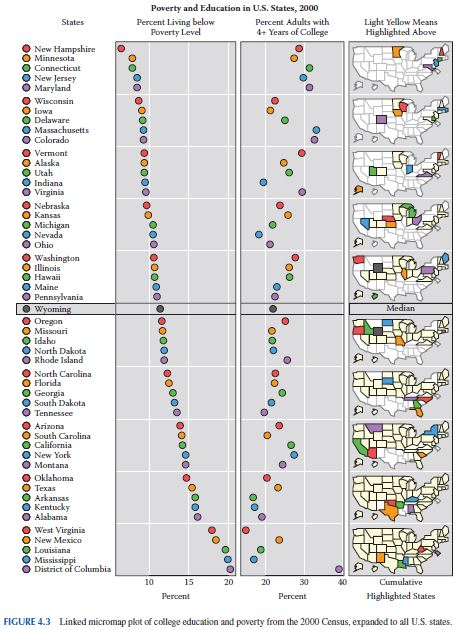
\includegraphics[width=0.9\textwidth]{hw02_CarrPickle_Fig_4_3.JPG}
\caption{Original Figure 4.3 from Carr \& Pickle (2010).}
\label{fig:OrigFig4.3}
\end{figure}


\end{enumerate}


\newpage


\item {\bf My Worst Color Choices Ever!} (25 Points): \\
You have to find one of your truly terrible, previously created R graphics with respect
to colors. This should come from your current or past undergraduate, MS,
or PhD research or from any of your HWs or projects for another class.
Graphics you created for some outside employer or internship also are acceptable.
Clearly indicate the source of this graphic.
There must be at least five different ``colors'' in this graphic
(other than black and white). If you claim that you never created any truly
terrible graphic with respect to colors, find such a bad graphic on the web,
e.g., Wikipedia, US Government web sites, etc. However, as a penalty,
such an external graphic must have at least eight different ``colors''
(other than black and white).

You have to work on  the following tasks:

\begin{enumerate}
\item (5 Points) Show your original graph and
describe what is bad  with respect to your previously selected colors. \\

\underline{Answer:} \\
{\scriptsize
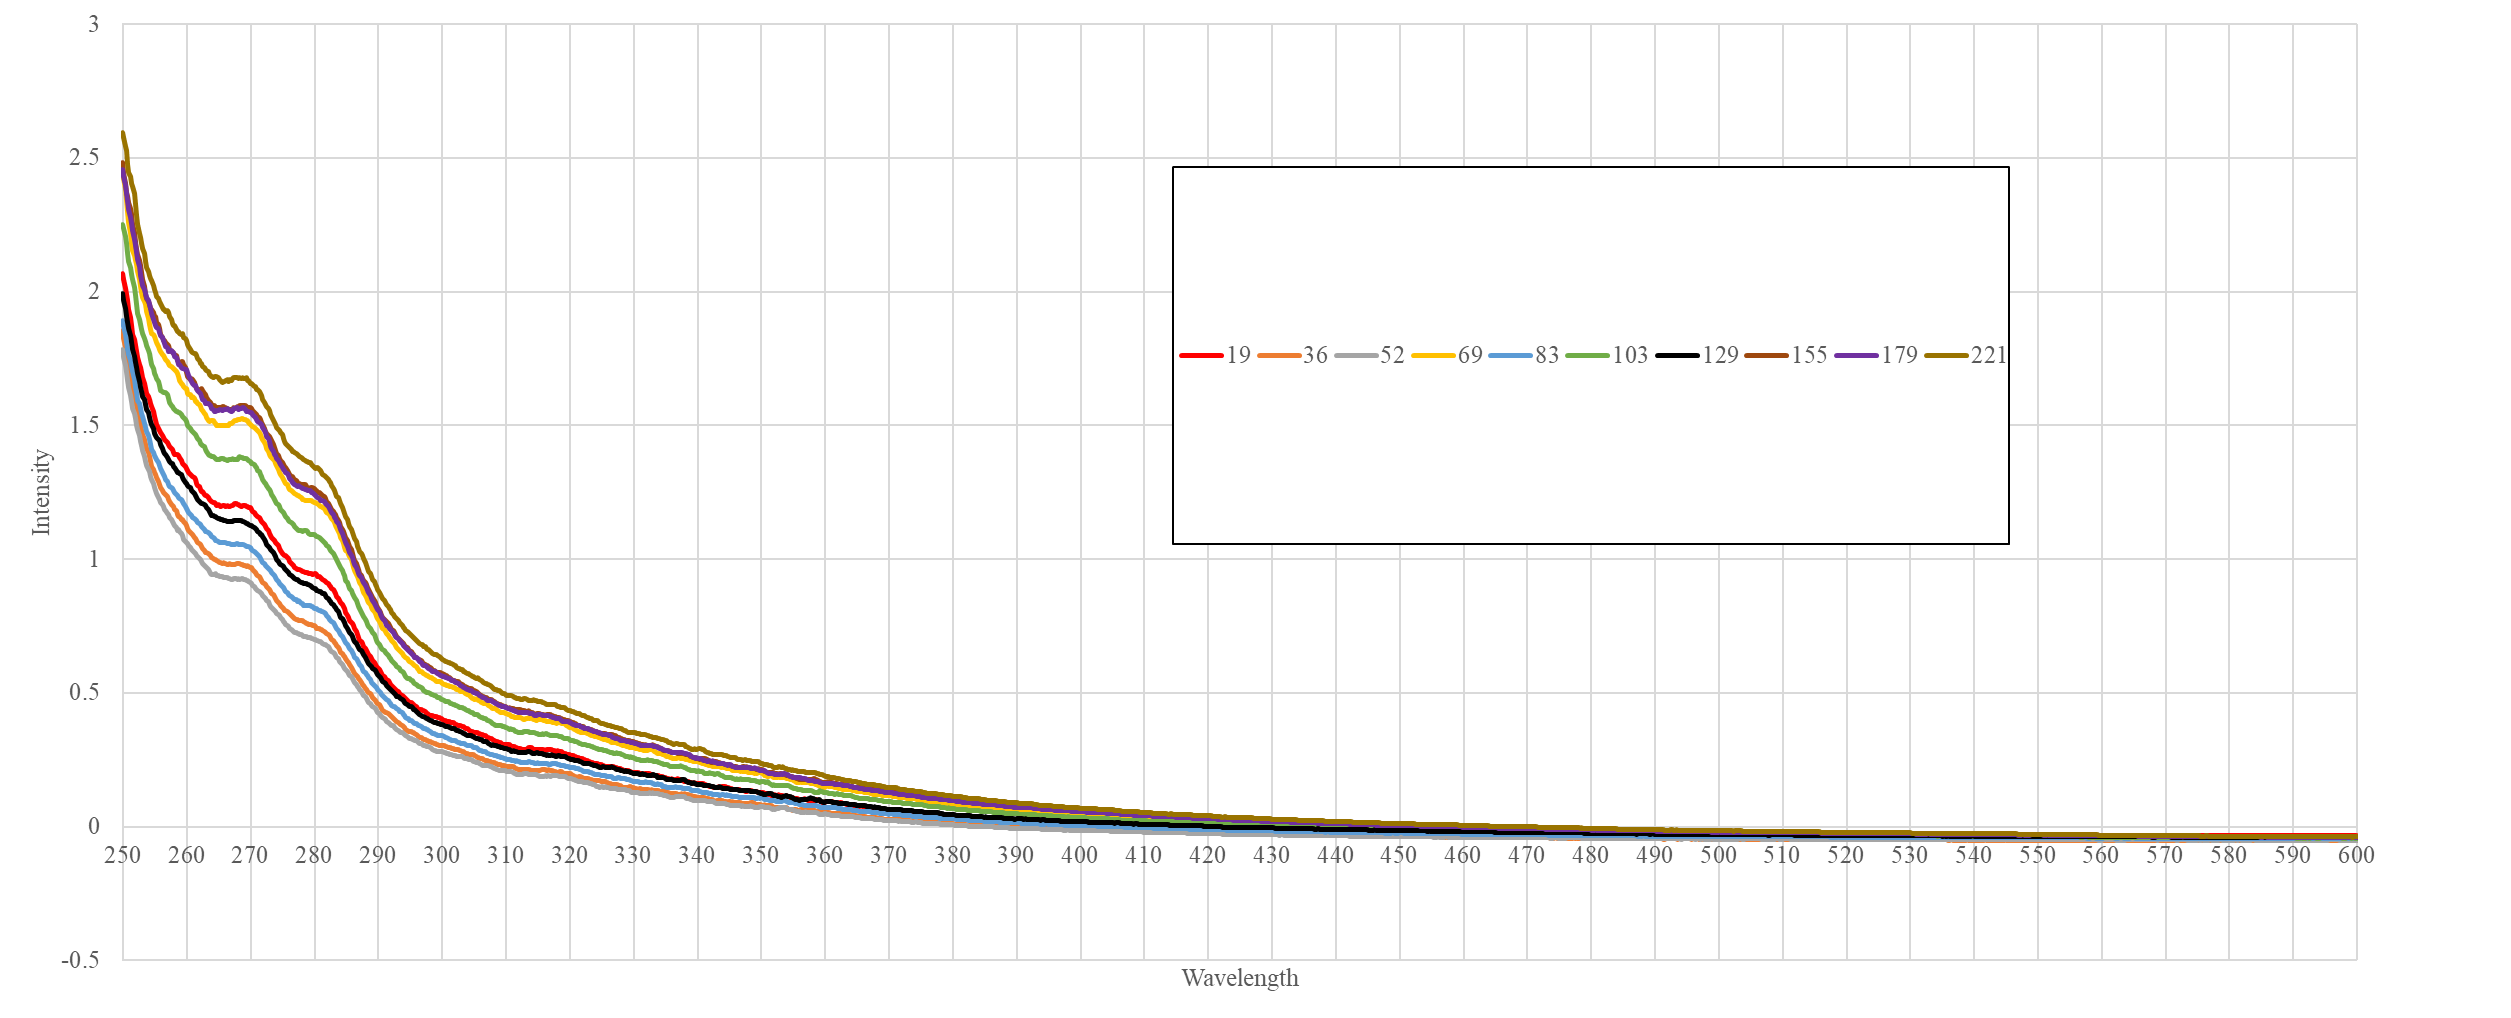
\includegraphics[width=.9\textwidth]{fionas_bad_graph.PNG}\\
This was a graph from a chemistry class (created in Microsoft Excel) measuring the UltraViolet  and Visual light spectroscopy of Cadmium-Selenium nanoparticles, where each line represents a measurement at a particular time in seconds (see legend). It may also be worth noting that the experiment itself failed, but a plot still needed to be constructed.  Several of the colors that were originally chosen were done to differentiate from one another, however upon reconsideration, are very difficult to differentiate for a color-impaired individual as the colors are very similar in intensity, and cover a wide variety of color spectrums.
}



\item (5 Points) Run your original figure through the nine color blindness
simulation modes at \\
{\small
\url{https://www.color-blindness.com/coblis-color-blindness-simulator/}} \\
and save the results. For which type of colorblindness (if any)
did  your original figure contain meaningful color information? \\

\underline{Answer:} \\

\begin{figure}[h]
\begin{center}$
\begin{array}{ccc}
  Original & Monochromacy & Achromatosia\\
  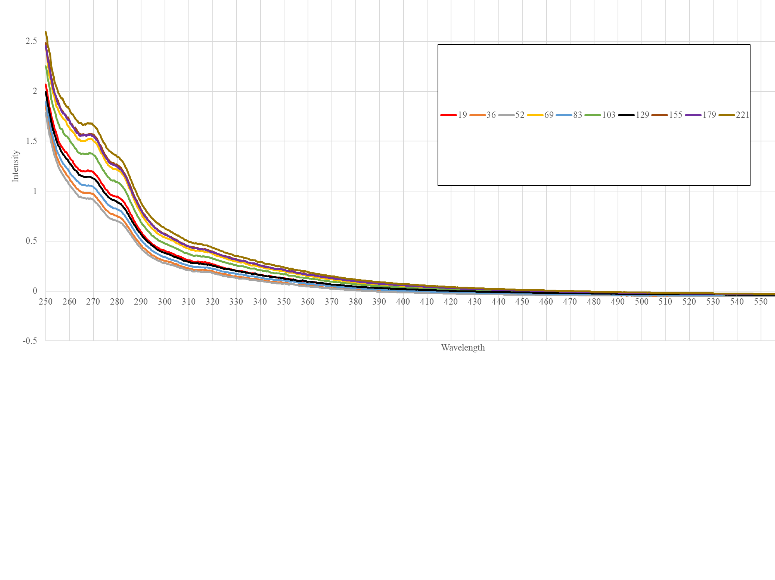
\includegraphics[width=.27\textwidth]{original_graph.PNG} &
  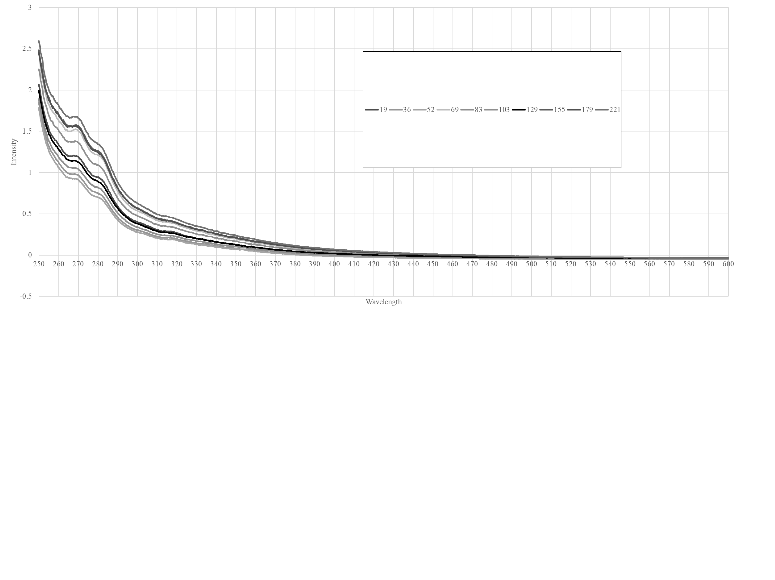
\includegraphics[width=.27\textwidth]{Monochromacy_graph.PNG} &
  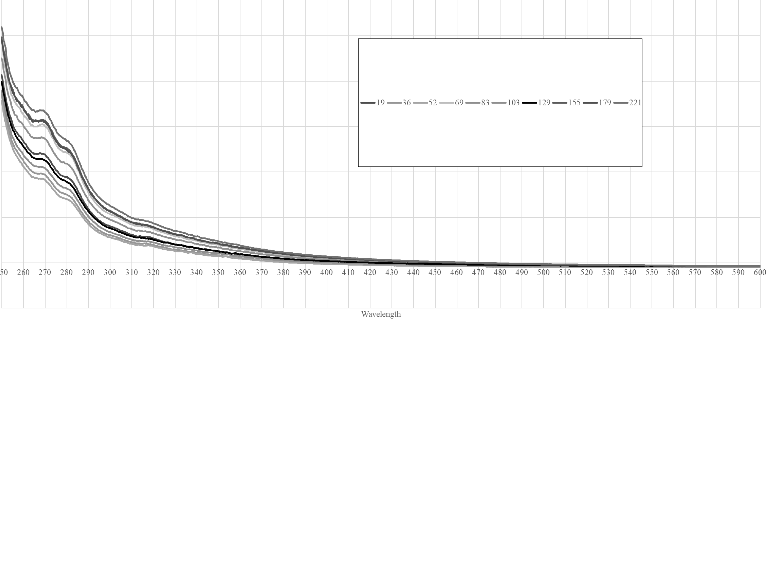
\includegraphics[width=.27\textwidth]{Achromatopsia_graph.PNG}\\
  Protanomaly & Deuteranomaly & Tritanomaly\\
  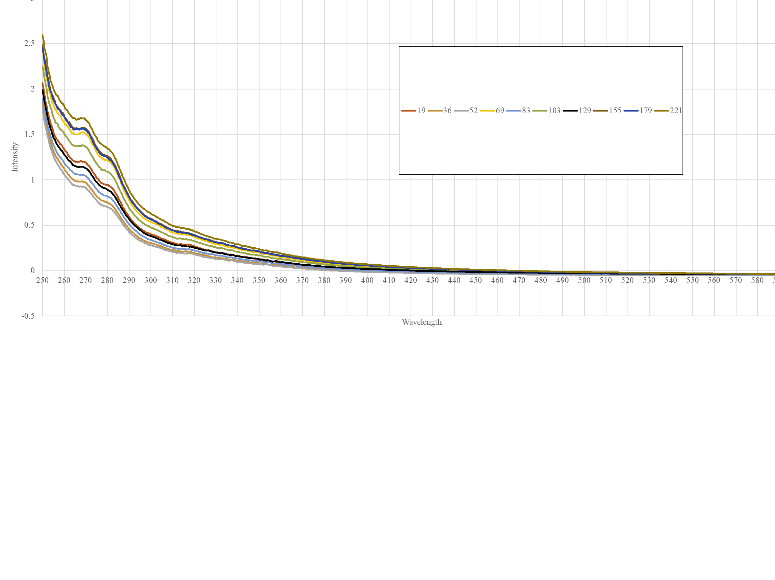
\includegraphics[width=.27\textwidth]{Protanomaly_graph.PNG} &
  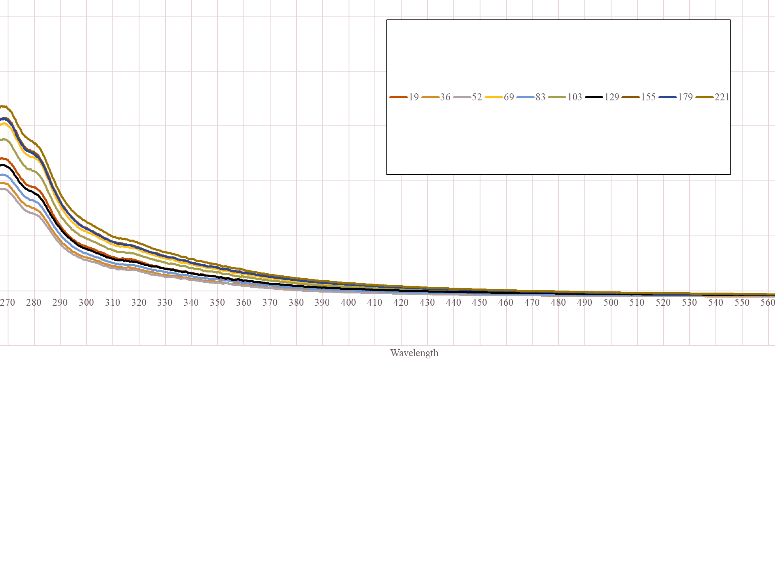
\includegraphics[width=.27\textwidth]{Deuteranomaly_graph.PNG} &
  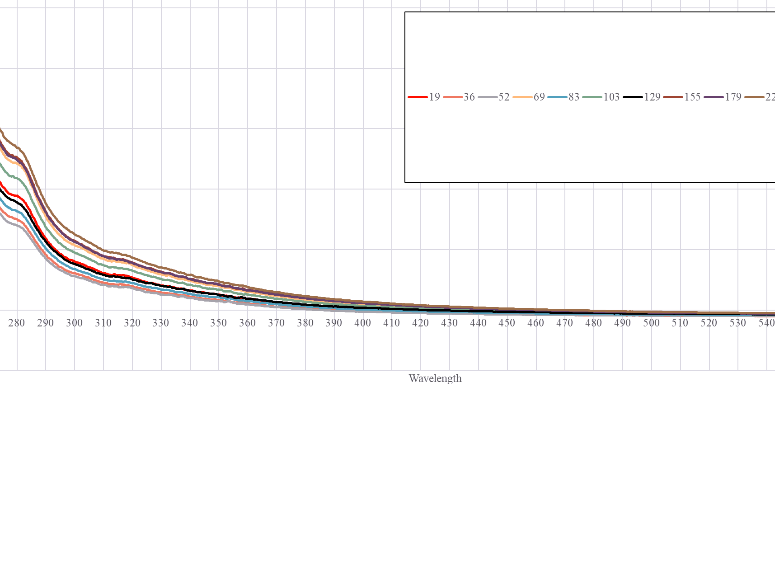
\includegraphics[width=.27\textwidth]{Tritanomaly_graph.PNG}\\
  Protanopia & Deuteranopia & Tritanopia\\
  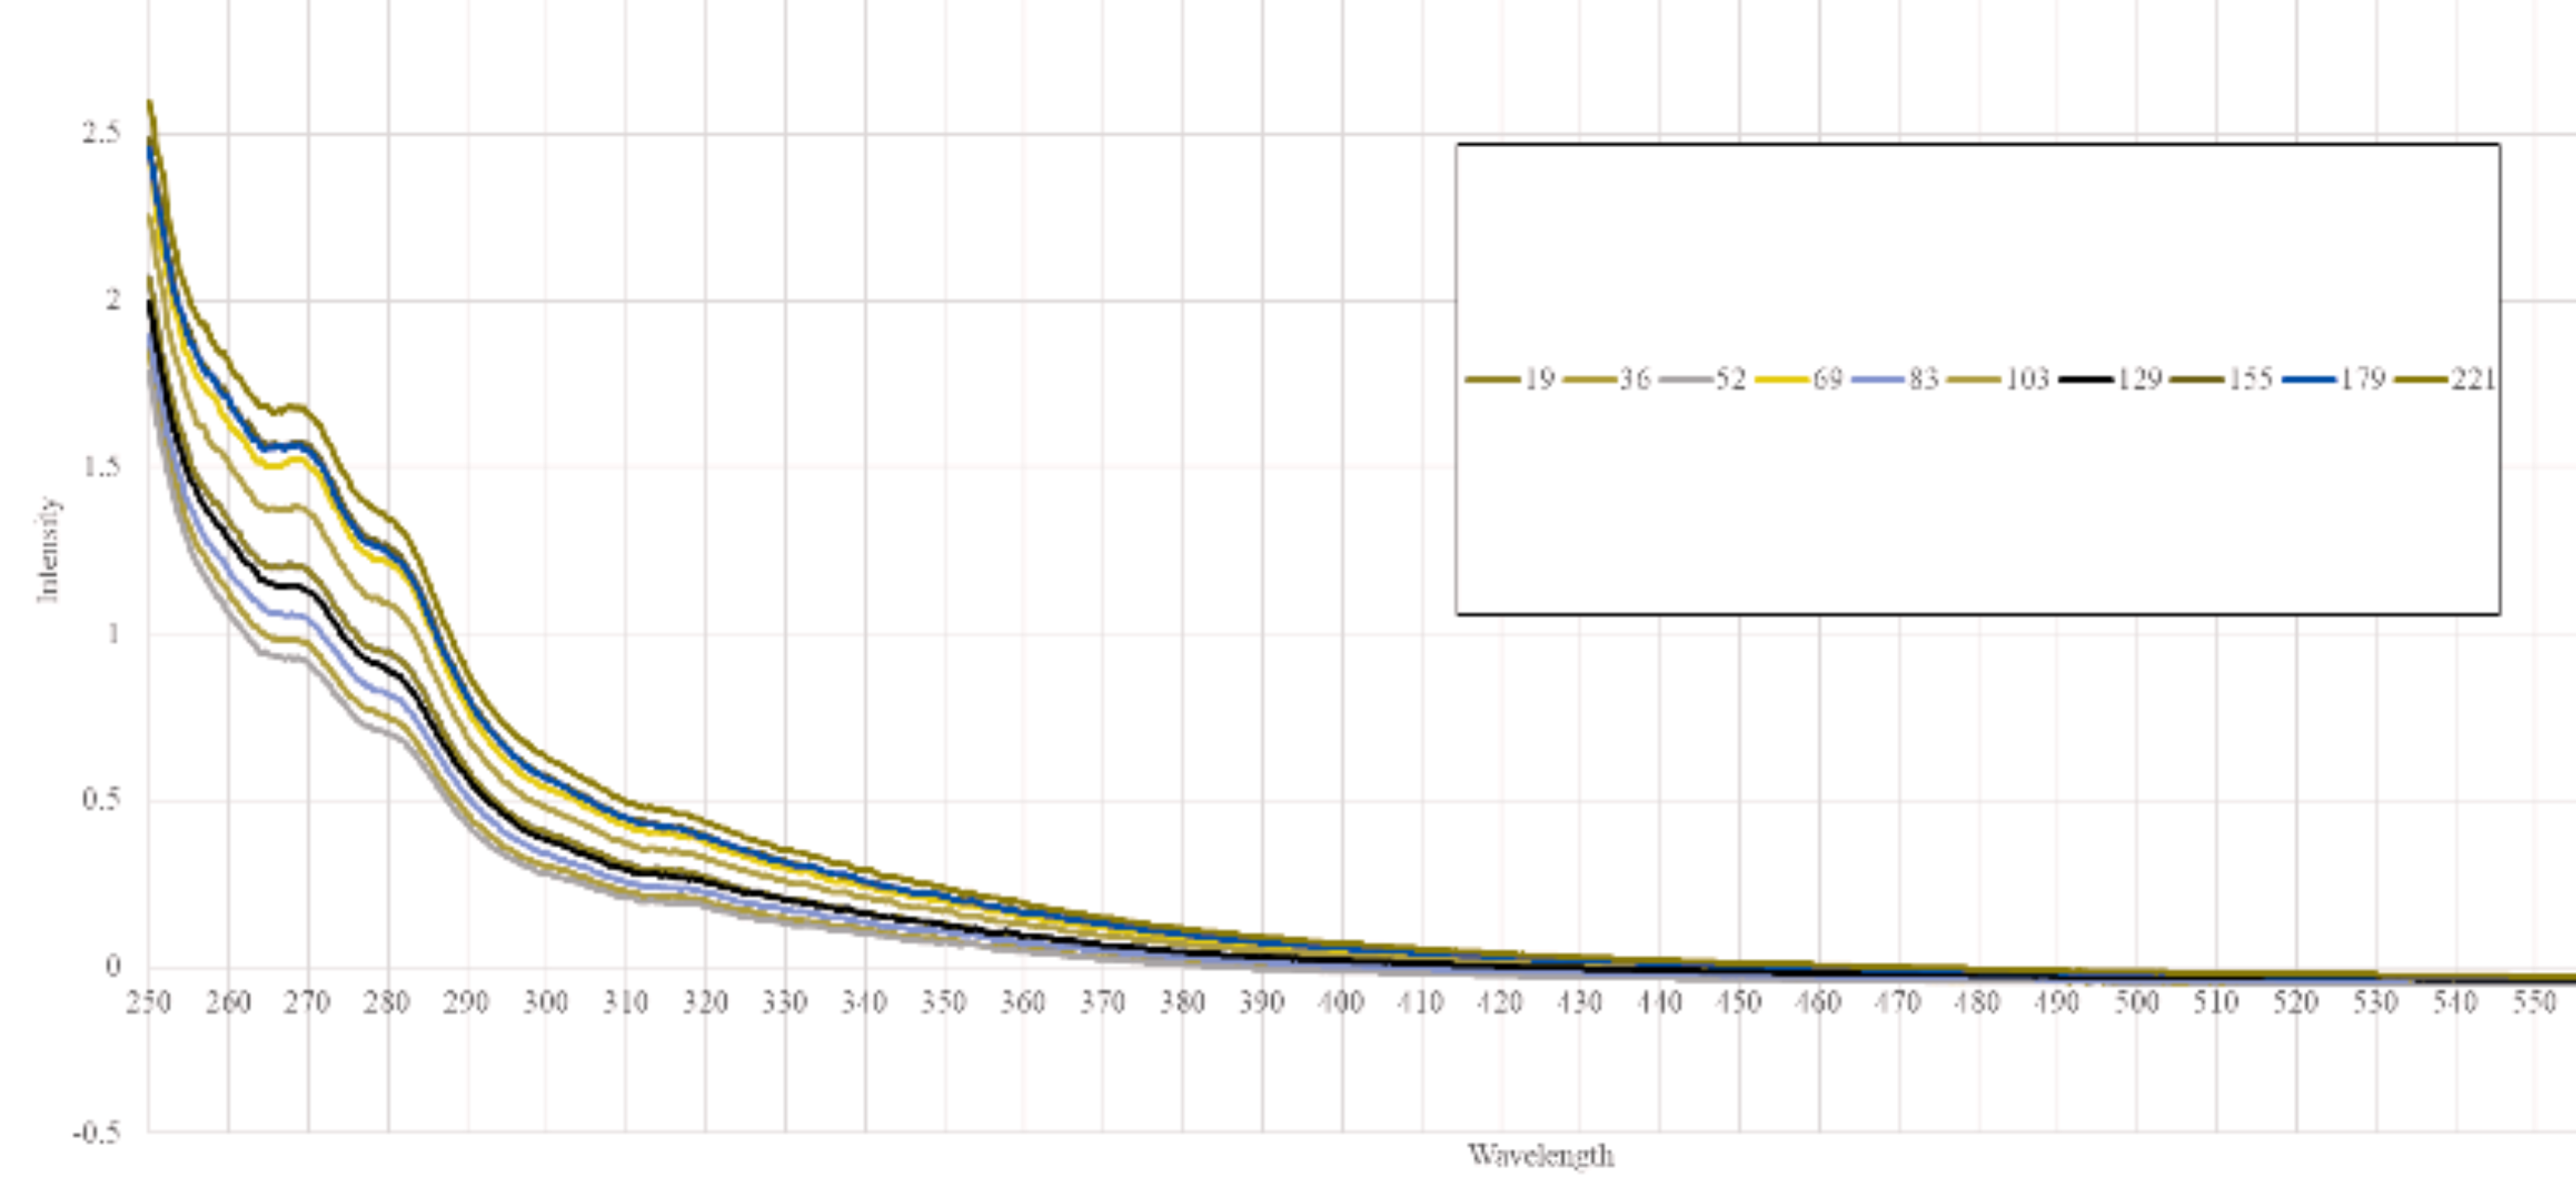
\includegraphics[width=.27\textwidth]{Protanopia_graph.PNG} &
  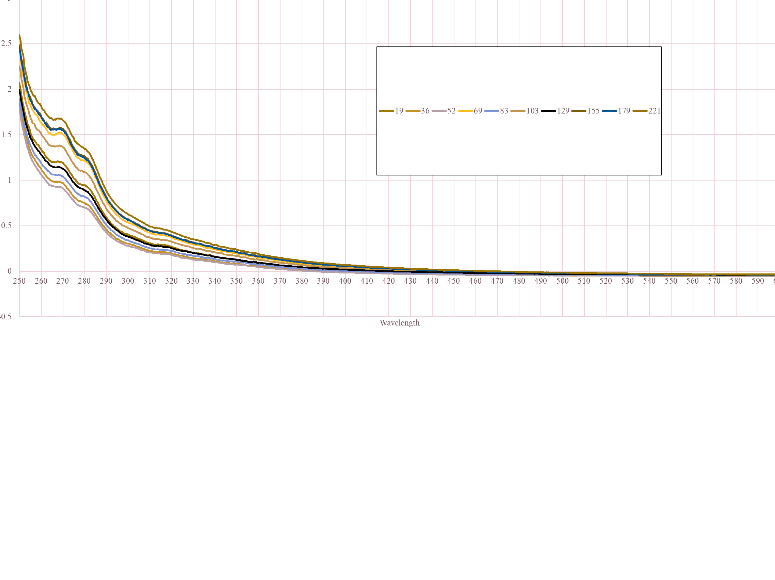
\includegraphics[width=.27\textwidth]{Deuteranopia_graph.PNG} &
  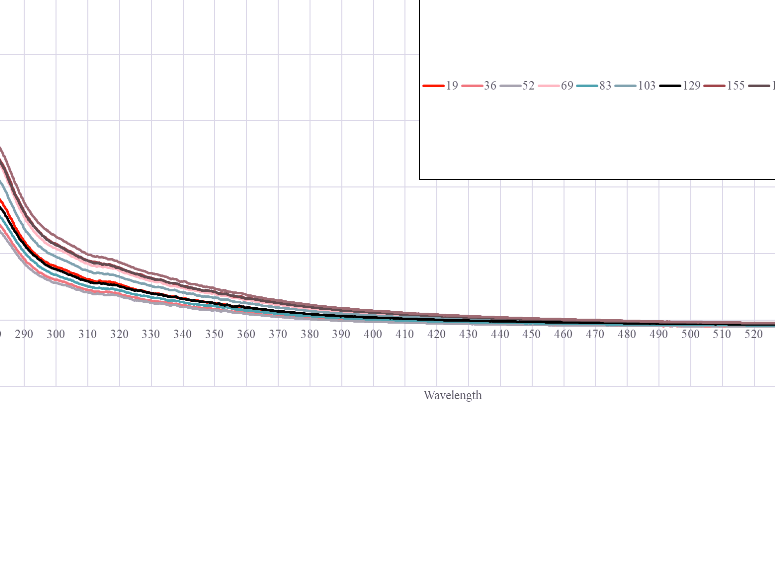
\includegraphics[width=.27\textwidth]{Tritanopia_graph.PNG}\\
\end{array}$
\end{center}
\end{figure}

{\scriptsize
Protanomaly, Tritanomaly, and (maybe) Tritanopia all retain the original information being contained in the graph.  All of the rest loose at least a third of the information from color.
}




\item (10 Points) Modify colors and any other design features (such as line styles,
line thickness, plotting symbols, shading, etc.) 
from your original figure to make it more suitable
for colorblind viewers. Check again with \\
{\small
\url{https://www.color-blindness.com/coblis-color-blindness-simulator/}}. \\
Iterate this step until you have found a satisfactory solution.
{\bf Show your R code and
include the final version of your figure and the final eight colorblindness simulations
as an answer to this question part.}

Be aware that there may be no perfect color choices for all of the simulated
colorblindness scenarios. However, if your colors still remain hard to distinguish,
your other design features should help to distinguish the different
elements in your improved graph. \\

\underline{Answer:}
{\scriptsize
\begin{Schunk}
\begin{Sinput}
> library(ggplot2)
> spectroscopy <- read.csv(file = "Spectroscopy.csv", header=TRUE, sep=",")
> better.col <- brewer.pal(10, "Spectral")
> ggplot(data = spectroscopy, aes(x=Wavelength)) + 
+   
+   geom_line(aes(y=t19, color = better.col[1])) +
+   geom_line(aes(y=t36, color = better.col[2])) +
+   geom_line(aes(y=t52, color = better.col[3])) +
+   geom_line(aes(y=t69, color = better.col[4])) +
+   geom_line(aes(y=t83, color = better.col[5])) +
+   geom_line(aes(y=t103, color = better.col[6])) +
+   geom_line(aes(y=t129, color = better.col[7])) +
+   geom_line(aes(y=t155, color = better.col[8])) +
+   geom_line(aes(y=t179, color = better.col[9])) +
+   geom_line(aes(y=t221, color = better.col[10])) +
+   
+   xlab("Wavelength (nm)") +
+   ylab("Absorbance") +
+   ggtitle("UV/Vis Spectoscopy of Cd-Se") +
+   scale_color_brewer(name="Time in \nSeconds",
+                       labels = c("19s","36s","52s","69s","83s","103s","129s","155s","179s","221s"), palette = "RdYlBu")+
+   xlim(250,600) +
+   #theme_minimal() + 
+   theme(legend.position = c(.8,.7), plot.title = element_text(hjust = 0.5))
\end{Sinput}
\end{Schunk}
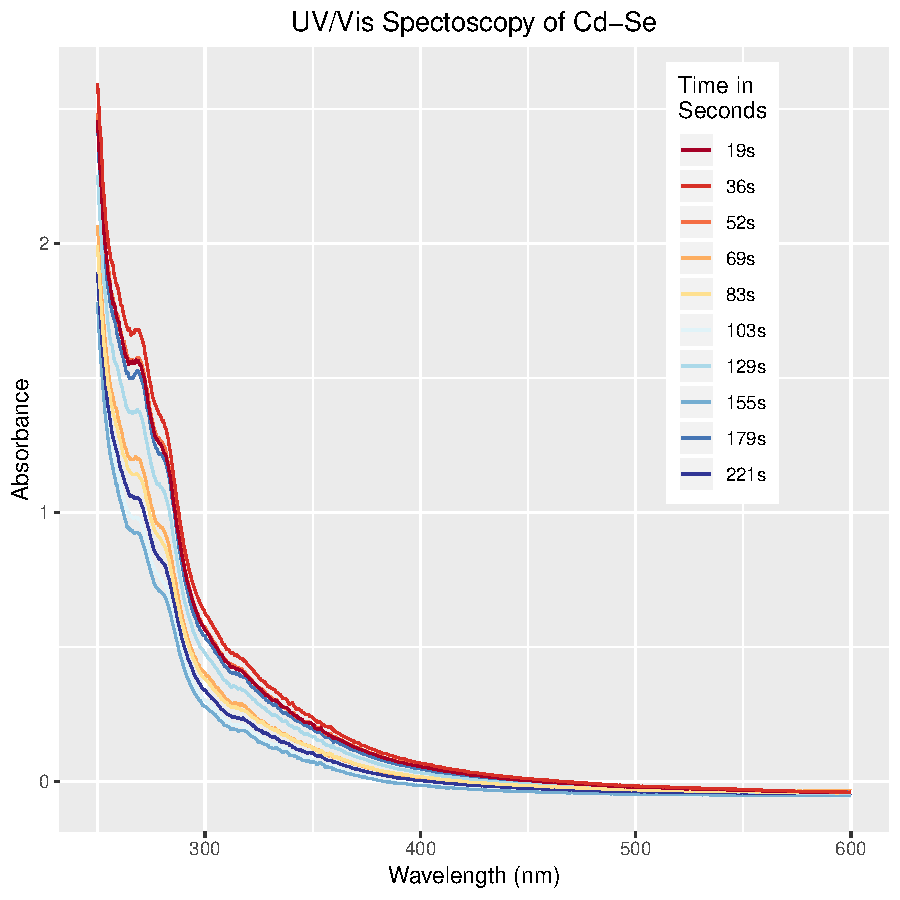
\includegraphics{hw02_bartschi-008}
}


\item (5 Points) Clearly describe how you have modified your figure to make
it more appropriate for colorblind viewers. Mention the names of the color
palette you used, how many colors you used, whether you omitted some colors
from this palette (e.g., just used 4 colors from a 5--color palette), etc.
Likely, it was not enough
to just choose a colorblind color palette from {\it RColorBrewer}.
Rather, additional changes may have been necessary. Do not forget to mention
these modifications as well. \\

\underline{Answer:} \\
{\scriptsize
The goal in using Color Brewer was to extend the number of individuals who would be able to view the graphic.  In using 10 bins of the {\it RdYlBu} color pallet, I was able to differentiate between each of the lines for nearly all forms of color blindness except for Achromatopsia or Monochromacy.  I found from trial and error that keeping all of the colors was typically best.  I also sought to make every other line dotted, but it ended up complicating the graph an unnecessary amount.  Ultimately, since there is little useful information to extract from this graphic to begin with due to the failed nature of the original experiment, it made it very difficult to choose a meaningful and useful color scheme, but I believe that the modifications that I have made have made the graph more friendly to color impaired individuals.
}

\end{enumerate}

\end{enumerate}


\newpage


\noindent{\Large \bf General Instructions}~\\


\begin{enumerate}
\item Create a single pdf document, using R Markdown, Sweave, or knitr.
When you take this course at the 6000--level, you have to use \LaTeX\ in
combination with Sweave or knitr.
You only have to submit this one document.

\item Include a title page that contains your name, your A--number, the number of
the assignment, the submission date, and any other relevant information.

\item Start your answers to each main question on a new page (continuing with the next
part of a question on the same page is fine). 
Clearly label each question and question part.

\item Show your R code for each question part!

\item Before you submit your homework, check that you
follow all recommendations from Google's R Style Guide
(see \url{https://google.github.io/styleguide/Rguide.xml}). 
Moreover, make sure that your R code is consistent, i.e., that you use the same
type of assignments and the same type of quotes throughout your entire homework.

\item Give credit to external sources, such as stackoverflow or help pages. Be specific
and include the full URL where you found the help (or from which help page you got 
the information). Consider R code from such sources as ``legacy code or third--party code'' 
that does not have to be adjusted to Google's R Style (even though it would be nice,
in particular if you only used a brief code segment).

\item {\bf Not following the general instructions outlined above will result in point deductions!}

\item For general questions related to this homework, please
use the corresponding discussion board in Canvas! I will try to
reply as quickly as possible. Moreover, if one of you knows
an answer, please post it. It is fine to refer to web pages
and R commands, but do not provide the exact R command with all required arguments
or which of the suggestions from a stackoverflow web page eventually worked for you! 
This will be the task for each individual student!

\item Submit your single pdf file via Canvas by the submission deadline.
Late submissions will result in point deductions as outlined on the syllabus.

\end{enumerate}


\end{document}

